\documentclass[tikz,crop]{standalone} %\usetikzlibrary{calc} 
\usepackage{rubikcube,rubikrotation,rubikpatterns,rubiktwocube} 
\newcommand{\CycleThreeEdgesFlipTwo}{[CycleThreeEdgesFlipTwo],F,R,U,Rp,Up,Fp}%
\newcommand{\cyclethreeedgesfliptwo}{\CycleThreeEdgesFlipTwo}%
%
%----corner sequences--------------------------
\newcommand{\AllYellow}{[allyellow],R,U,Rp,U,R,Up,Up,Rp}% = SUNE  %cross -->allyellow
\newcommand{\allyellow}{\AllYellow}%
\newcommand{\CycleThreeCorners}{[cyclethreecorners],Lp,U,R,Up,L,U,Rp,Up}%
\newcommand{\cyclethreecorners}{\CycleThreeCorners}%
\newcommand{\cornerrotate}{[cornerrotate],Up,Rp,Dp,R,U,Rp,D,R}
\newcommand{\SwapTwoCorners}{[swaptwocorners],Rp,F,Rp,B2,R,Fp,Rp,B2,R2,Up}
\newcommand{\swaptwocorners}{\SwapTwoCorners}
%
%% brace and bracket macros 
\newcommand{\Rubikbracket}[1]{$\left(\mbox{#1}\right)$}
\newcommand{\Rubikbrace}[1]{$\left\{\mbox{#1}\right\}$}
\newcommand{\cubenumber}[1]{\strut\raisebox{1cm}{#1}}
\begin{document}
\begin{figure}
\begin{center}
	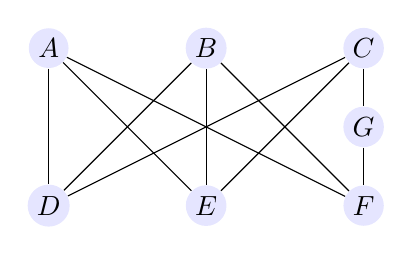
\begin{tikzpicture}
  [scale=2,auto=left,every node/.style={circle,inner sep=1.5pt, fill=blue!10}]
  \node (n1) at (0.0000000,  1.0000000) {$A$};
  \node(n2) at (1,1)  {$B$};
  \node (n3) at (2,1)  {$C$};
  \node (n4) at (0,0) {$D$};
  \node (n5) at (1,0) {$E$};
  \node (n6) at (2,0) {$F$};
  \node (n7) at (2,0.5) {$G$};
%  \node (n5) at (0,0)  {$E$};
%  \node (n6) at (0.25, -0.7)  {$F$};
%  \node (n7) at (1,-0.7) {$G$};
%  \node (n8) at (2,-0.7)  {$H$};
%  \node (n9) at (1,0)  {$I$};
%  \node(n10) at (2,0)  {$J$};

  \foreach \from/\to in {n1/n4, n1/n5, n1/n6, n2/n4, n2/n5, n2/n6, n3/n4, n3/n5, n3/n7, n7/n6}
    \draw (\from) -- (\to);
\end{tikzpicture}
%\caption{An additional vertex and edge appended to $C_9$.}\label{fig:newgraph}
\end{center}
\end{figure}
\end{document}